\begin{exmp}
\subsubsection*{Transmission line analysis using a Smith chart}
A 50$\Omega$ line is terminated in a load impedance $25+j35\Omega$. Find the following using a Smith chart.
\begin{enumerate}[(a)]
\item Reflection coefficient in cartesian and polar form,
\item Reflection coefficient and impedance at a distance of $0.2\lambda$ from the load end of the line.
\item VSWR on the line.
\end{enumerate}

\subsubsection*{Solution}
We are given $Z_{L}=25+j35\varOmega$ and $Z_{0}=50\varOmega$, so first, we normalize the load impedance
\begin{dmath*}
\bar{Z_{L}}=\frac{25+j35}{50}=0.5+j0.7
\end{dmath*}
We mark this point on the Smith chart as shown in figure~\ref{fig:workedexample2}.
\begin{figure}[h]
\centering
\includegraphics[width=1\linewidth]{\pathtopartone/graphics/"Smith chart 1"}
\caption{Worked Example}
\label{fig:workedexample2}
\end{figure}

To get the reflection coefficient, we draw a circle from the origin of the Smith chart through the marked point (normalized load impedance), A. The distance between point A and the centre gives the magnitude of the reflection coefficient\footnote{
The distance is read from the scale for reflection coefficient E or I at the bottom of the Smith chart page

\underline{Note}: This method is different from that used in example~\ref{exmp:locatepoints} and both methods are correct
}. We read the value as
\begin{align*}
|\Gamma_{L}| = 0.52
\end{align*}

To determine the angle $\phi_{L}$, we draw a straight line from the origin through point A to the outermost circle as shown in figure~\ref{fig:workedexample2}. From the scale that reads \textquotedblleft ANGLE OF REFLECTION COEFFICIENT\textquotedblright\;, read the angle the line makes from the positive real axis. The value gives the angle of the reflection coefficient in polar form so that the reflection coefficient at the load is $0.52\angle100^o$ in polar form.

The cartesian form is obtained by converting the polar form to the cartesian form as shown below
\begin{align*}
\Gamma_{L} &= 0.52\angle100^o\\
&= 0.52e^{j100}\\
&= 0.52{\cos100 + j\sin100}\\
&= -0.09+j0.512
\end{align*}

The next step is to get the reflection coefficient at a distance of $0.2\lambda$ from the load point, that is, $\Gamma(0.2\lambda)$. 

First, we identify the scale on the outermost circle that reads \textquotedblleft WAVELENGTH TOWARDS GENERATOR\textquotedblright\; and measure the value measured at point A which we obtained as $0.11\lambda$. To move a distance $0.2\lambda$ towards the generator means to move clockwise along the scale\footnote{
Similarly, moving towards the load on the Smith chart means to move in the anticlockwise direction along the scale that reads \textquotedblleft WAVELENGTH TOWARDS LOAD\textquotedblright\;.
}. We mark this point as B, which has the value $0.11\lambda + 0.2\lambda=0.31\lambda$. We draw a straight line through the origin of the Smith chart and point B and determine the point of intersection with the VSWR circle. The point is marked P (see figure~\ref{fig:workedexample2}) which is the point of the reflection coefficient moved $0.2\lambda$ towards the generator. 

Recall the magnitude of the reflection coefficient is given by the distance between the centre and the point P and the angle is measured from the positive real axis. We read the value as
\begin{align*}
\Gamma(0.2\lambda) = 0.52\angle316^o
\end{align*}

To find the normalized impedance at point P, we locate the constant resistance and reactance circles through the point. In our case we obtained
\begin{align*}
\bar{Z}=1.4-j1.37\\
\text{Thus, }Z &=Z_{0}\times\bar{Z}\\
&= 50(1.4-j1.37)\\
&= 70-j68.5\varOmega
\end{align*}

Next, we obtain the value $\rho$ by reading the value at the rightmost side of the VSWR circle (see figure~\ref{fig:workedexample2}).
\begin{align*}
VSWR, \rho = 3.8
\end{align*}
\end{exmp}

\begin{exmp}
\subsubsection*{Transmission line analysis with Admittances}
A line is terminated in a normalized admittance $0.2-j0.5\varOmega$. Find 
\begin{enumerate}[(a)]
\item the location of the voltage maximum from the load end. 
\item the reflection coefficient, normalized admittance and normalized impedance at a distance $0.12\lambda$ from the load.
\end{enumerate}

\subsubsection*{Solution}
Now, in this problem, we are dealing with admittances instead of impedances. The admittance we are given here is already normalized, so we mark the point, $\bar{Y} = 0.2 - j0.5$, on the Smith chart as shown in figure~\ref{fig:workedexample3}.
\begin{figure}[h]
\centering
\includegraphics[width=1\linewidth]{\pathtopartone/graphics/"smith chart 3"}
\caption{Worked Example}
\label{fig:workedexample3}
\end{figure}

Next, we draw a circle from the origin of the Smith chart through that point $\bar{Y}_L$ which should help us determine the position of maximum voltage and reflection coefficient, normalized admittance and normalized impedance at $0.12\lambda$ from the load.

\subsubsection*{(a) Location of the voltage maximum from the load end}
For the admittance Smith chart, the voltage maximum will now lie on the leftmost side of the VSWR circle of the Smith chart. This point is marked as $V_\max$ on the Smith chart (see figure~\ref{fig:workedexample3}). The distance between $\bar{Y}_L$ and $V_\max$ on the Smith chart is the location of the voltage maximum moving towards the generator\footnote{
Recall we move clockwise when moving towards the generator.
}.

\subsubsection*{(b) Reflection coefficient, normalized admittance and impedance at a distance $0.12\lambda$ from the load}
First, we note the distance corresponding to $\bar{Y}_L$ which we measured as $0.424\lambda$ on the Smith chart. Moving a distance of $0.12\lambda$ towards the generator implies the new location is $0.424\lambda + 0.12\lambda = 0.544\lambda$. But the highest value on the wavelength scale is $0.5\lambda$ so the value on the scale which corresponds to $0.544\lambda$ is $0.044\lambda$\footnote{
$0.544\lambda-0.5\lambda$
}. Next, we draw a line from the origin of the Smith chart through that point and mark the point of intersection of the line with the VSWR circle as $\bar{Y}$ (see figure~\ref{fig:workedexample3}). We read the corresponding value of normalized admittance as:
\begin{align*}
\bar{Y} = 0.18 + j0.28
\end{align*}

To get the normalized impedance at the distance of $0.12\lambda$ from the load point, we transform the admittance by $\frac{\lambda}{4}$\footnote{
Recall that the normalized impedance inverts itself every $\frac{\lambda}{4}$
}. Put differently, the normalized admittance is the reciprocal(inverse) of the normalized impedance. A transformation by $\frac{\lambda}{4}$ can easily be calculated on the Smith chart by drawing a straight line from the normalized admittance, $\bar{Y}$ through the origin such that it divides the Smith chart into halves. We mark this point as $\bar{Z}$ (see figure~\ref{fig:workedexample3}) which is 180\textdegree from the point $\bar{Y}$. This point reads the values of normalized impedance as:
\begin{align*}
\bar{Z} = 1.6 - j2.6
\end{align*}

Finally, we need to measure the reflection coefficient. To get the magnitude, we measure the distance between the origin of the Smith chart and $\bar{Z}$\footnote{
This is done either with a pair of dividers preferably to take the length and read its distance on the scale at the bottom of the Smith chart page. Alternatively, divide the distance measured with a pair of dividers by the distance measured for the $r = 1.0$ constant resistance circle.
}. While we get the phase angle by measuring the angle suspended for the positive real axis. That is,
\begin{align*}
\Gamma = 0.7\angle328^o
\end{align*}
All these demonstrate are the effectiveness of the Smith chart in moving from impedance to admittance and vice versa. We switch from impedance to admittance by diagonally switching on the Smith chart. That is, at the load point for instance, $\bar{Y_{L}}$, if we go diagonally opposite, we get $\bar{Z_{L}}$. So basically, it helps us invert complex numbers. 
\end{exmp}

\subsection{Identifying Types of Load from Standing Wave Pattern\index{standing wave pattern}}\label{lec:lec9}

We have so far discussed how to solve some simple common transmission line problems using both impedances and admittances and then we discussed the constant VSWR circle. In this section, we will discuss how to identify the types of load from standing wave patterns. Standing wave pattern has two important characteristics which are:
\begin{enumerate}[(i)]
\item The location of maximum and minimum (current/voltage)
\item The VSWR circle.
\end{enumerate}
So \emph{how can we quickly identify the type of load\footnote{The type of load is not the exact value of the load} without calculating the VSWR?}

Recall that:
\begin{align}
VSWR = \frac{|V|_\max}{|V|_\min}
\label{eqn:vswr09}
\end{align}
From the equation~\eqref{eqn:vswr09}, the smaller the value of $|V|_\min$, the larger the value of ${VSWR}$, that is, as $|V|_\min$ tends to zero, ${VSWR}$ tends to infinity. When $|V|_\max{\approx}|V|_\min$, then $VSWR = 1$.

First, let us observe the variation of the impedance on the transmission line with the Smith chart then we will revisit our early question. Figures~\ref{fig:group91} and~\ref{fig:group92} are simplified Smith charts showing the VSWR circle for inductive and capacitive load at the top and bottom areas respectively.
\begin{figure}[h]
\centering
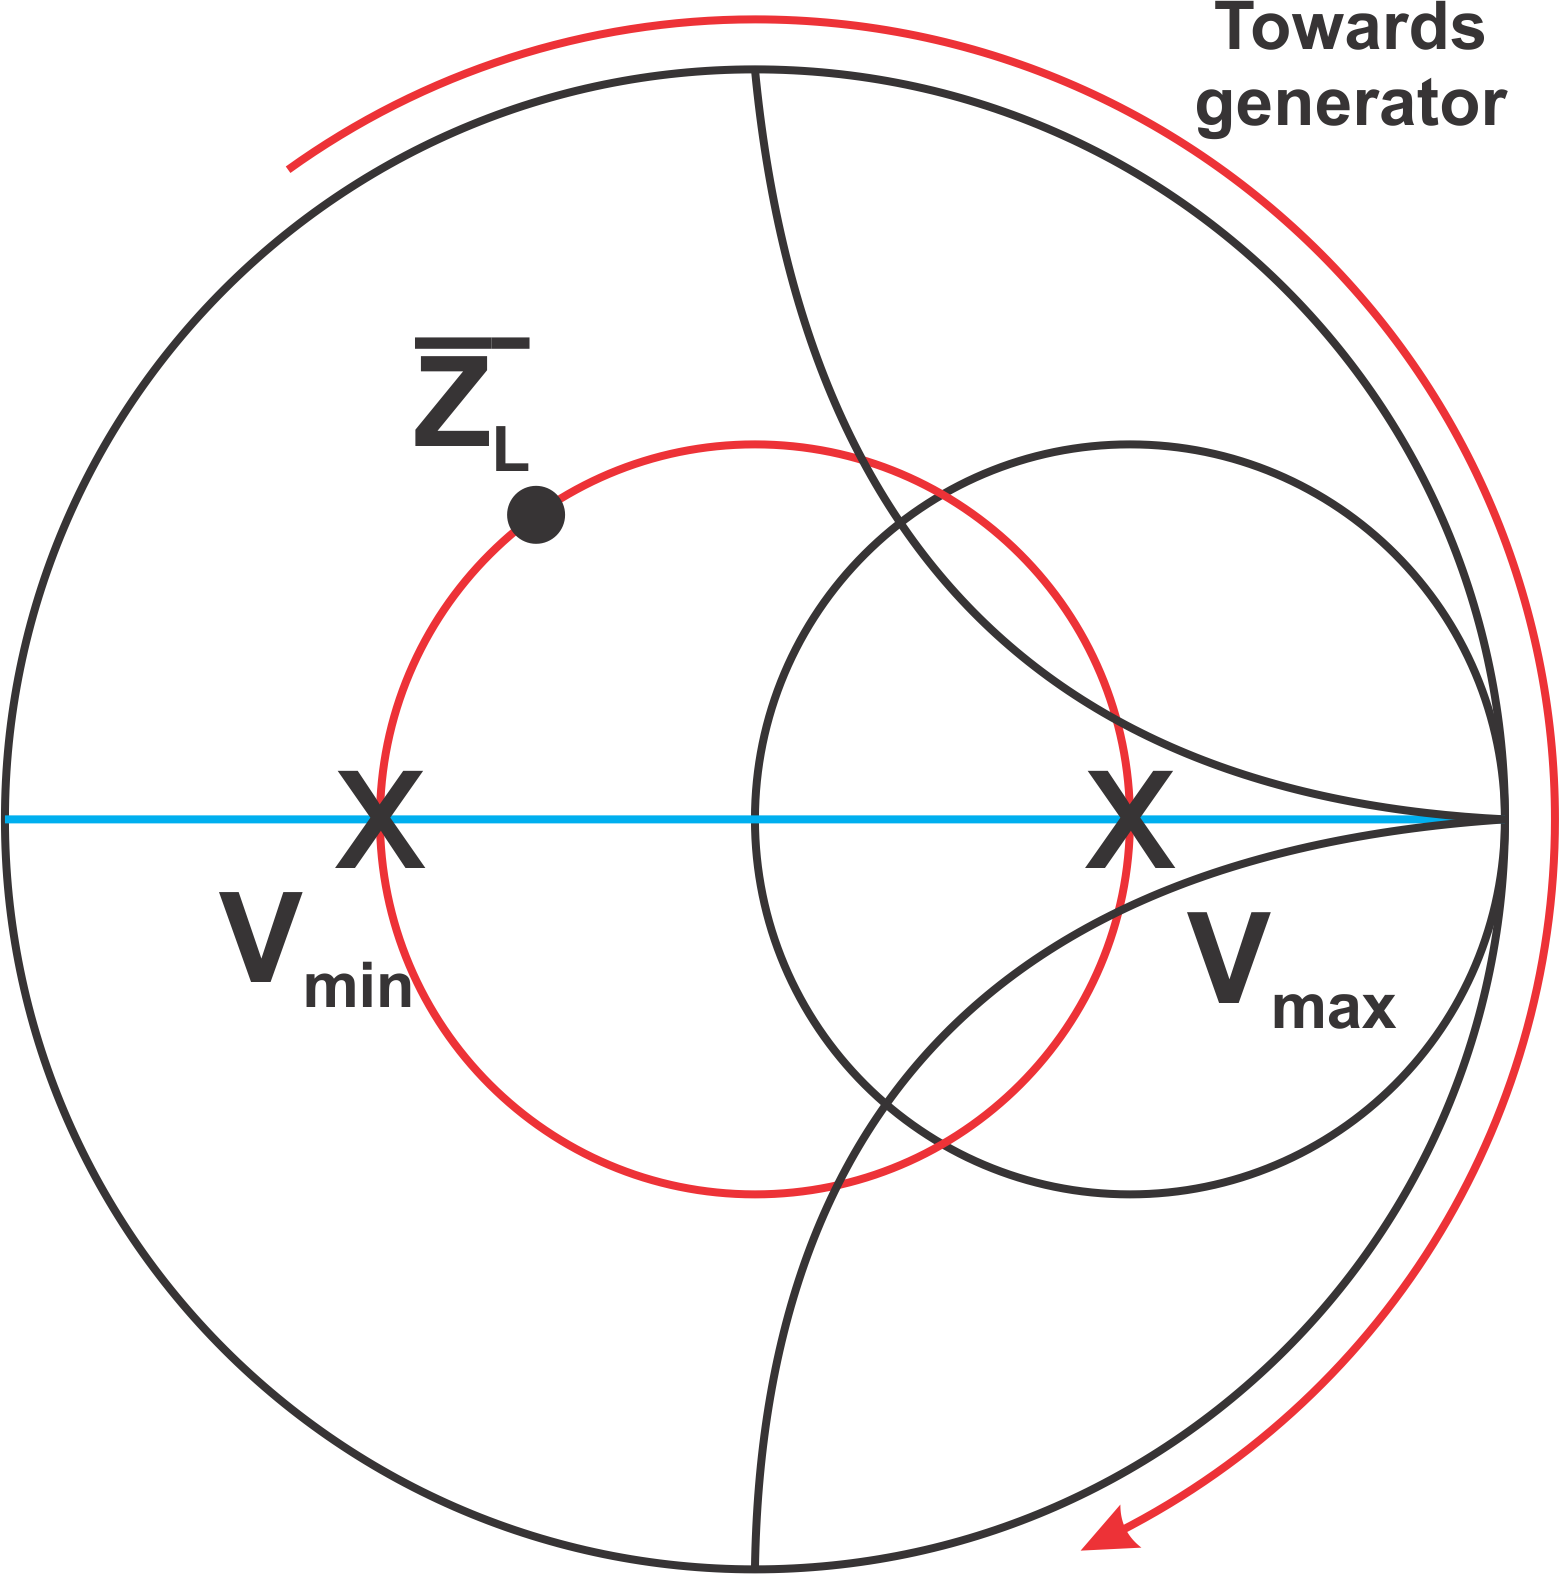
\includegraphics[scale=0.4]{\pathtopartone/graphics/Group91}
\caption{A Smith chart representation of inductive load}
\label{fig:group91}
\end{figure}
\begin{figure}[h]
\centering
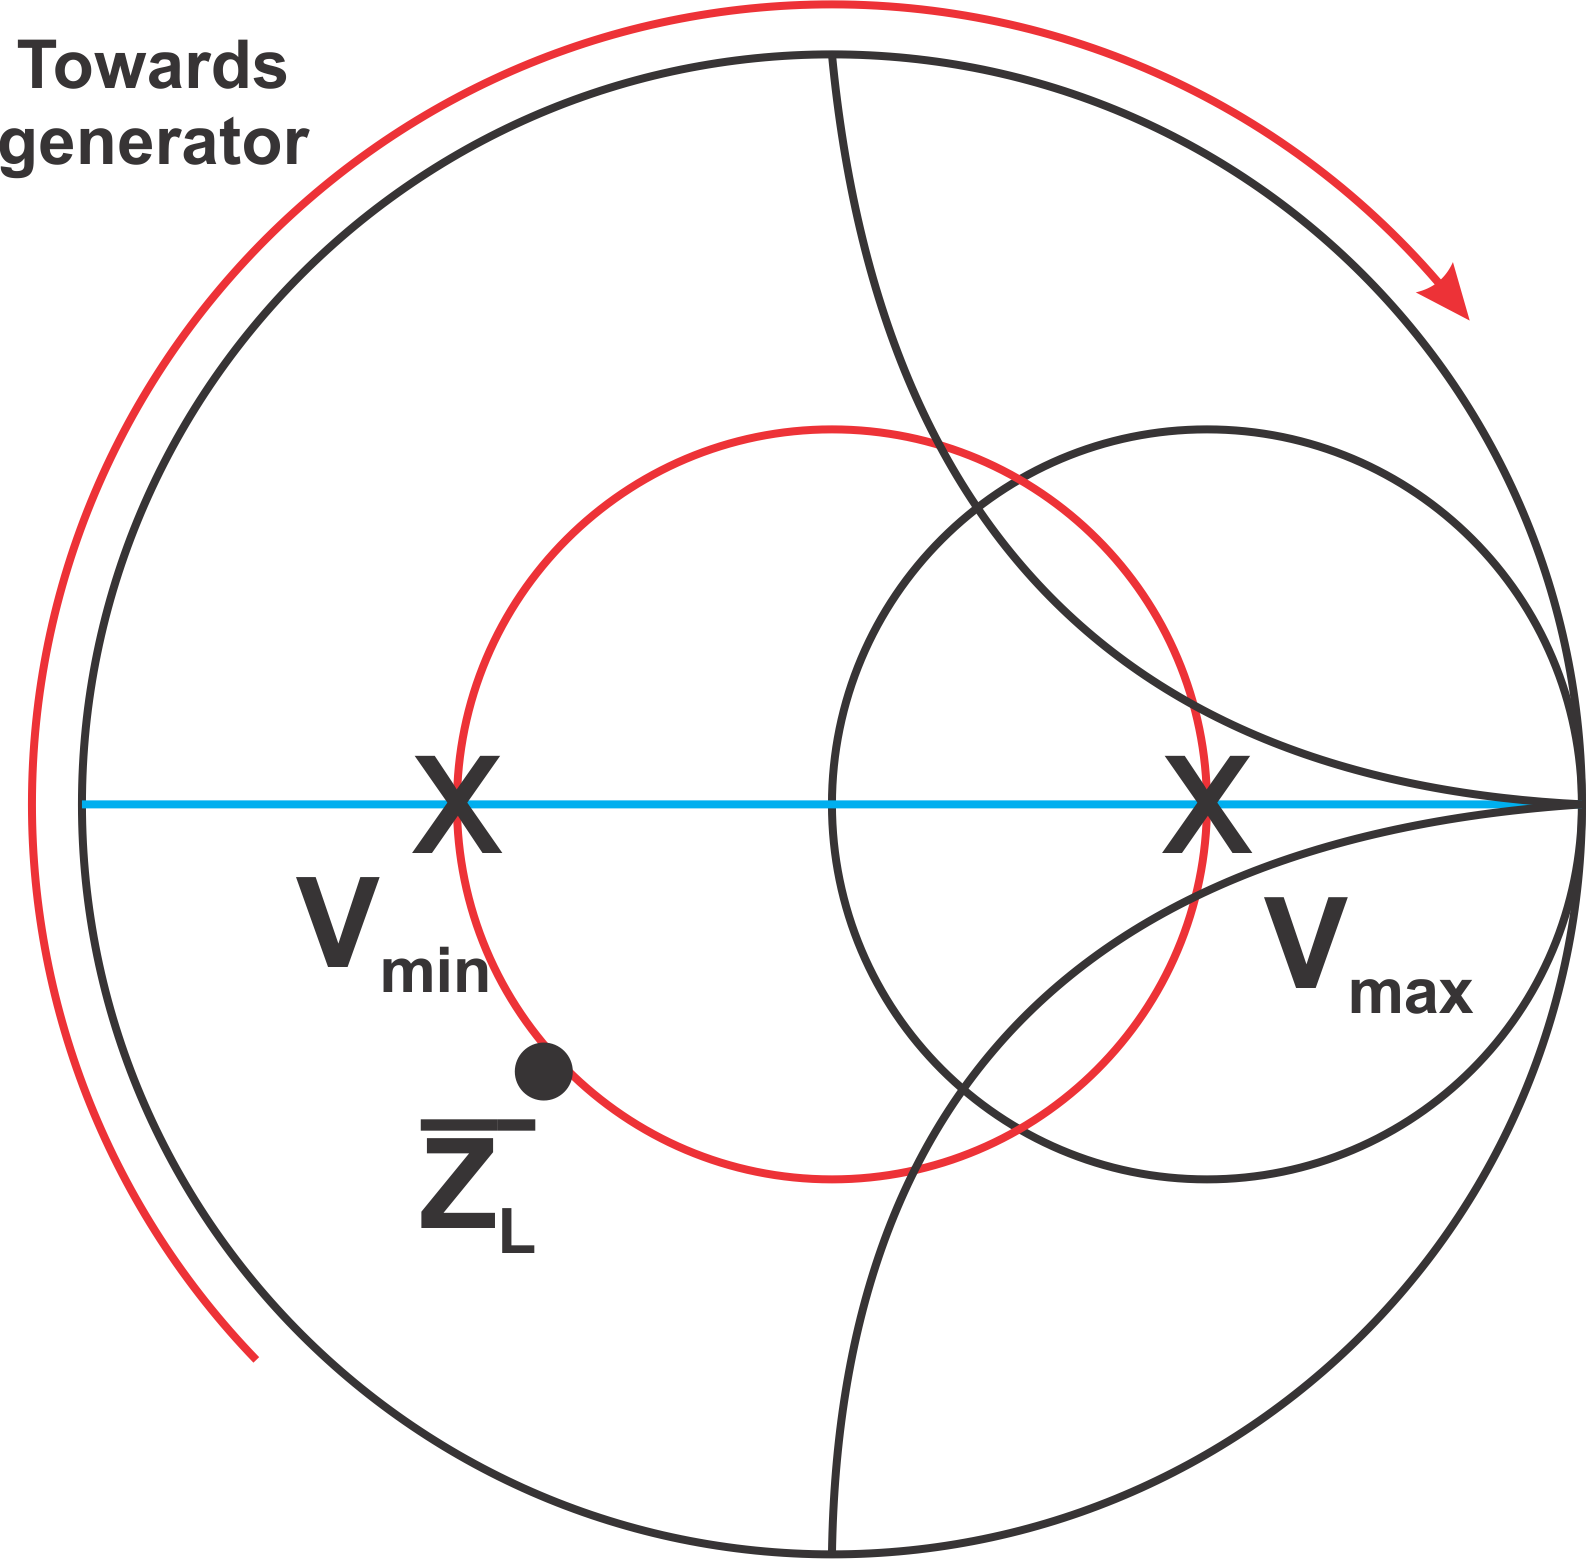
\includegraphics[scale=0.4]{\pathtopartone/graphics/Group92}
\caption{A Smith chart representation of capacitive load}
\label{fig:group92}
\end{figure}

As shown in figure~\ref{fig:group91}, if we move from the load towards the generator, that is, a clockwise rotation, for the inductive load we encounter $V_\max$ first before ${V_\min}$ in another $\frac{\lambda}{4}$ or $\pi rad$ movement. Similarly, if we move from $\bar{Z_L}$ in clockwise direction for capacitive load, we encounter $V_\min$ first before $V_\max$, in another $\frac{\lambda}{4}$ or $\pi rad$ movement. Also, $V_\min\neq0$ which means that for a complex inductive load that is not purely reactive, $VSWR\neq\infty$.

\subsubsection{Complex Reactive Loads}
Now, let us analyze some standing wave graphs and determine the type of load which they represent. The transmission line circuit is shown in figure~\ref{fig:group93} and we can analyse the standing wave pattern based on the new observation we have discussed. As the standing wave pattern moves from load towards the generator from right to left, it gets to a maximum first and its minimum is not zero so it $|V_\min|$ does not touch the real axis.
\begin{figure}[h]
\centering
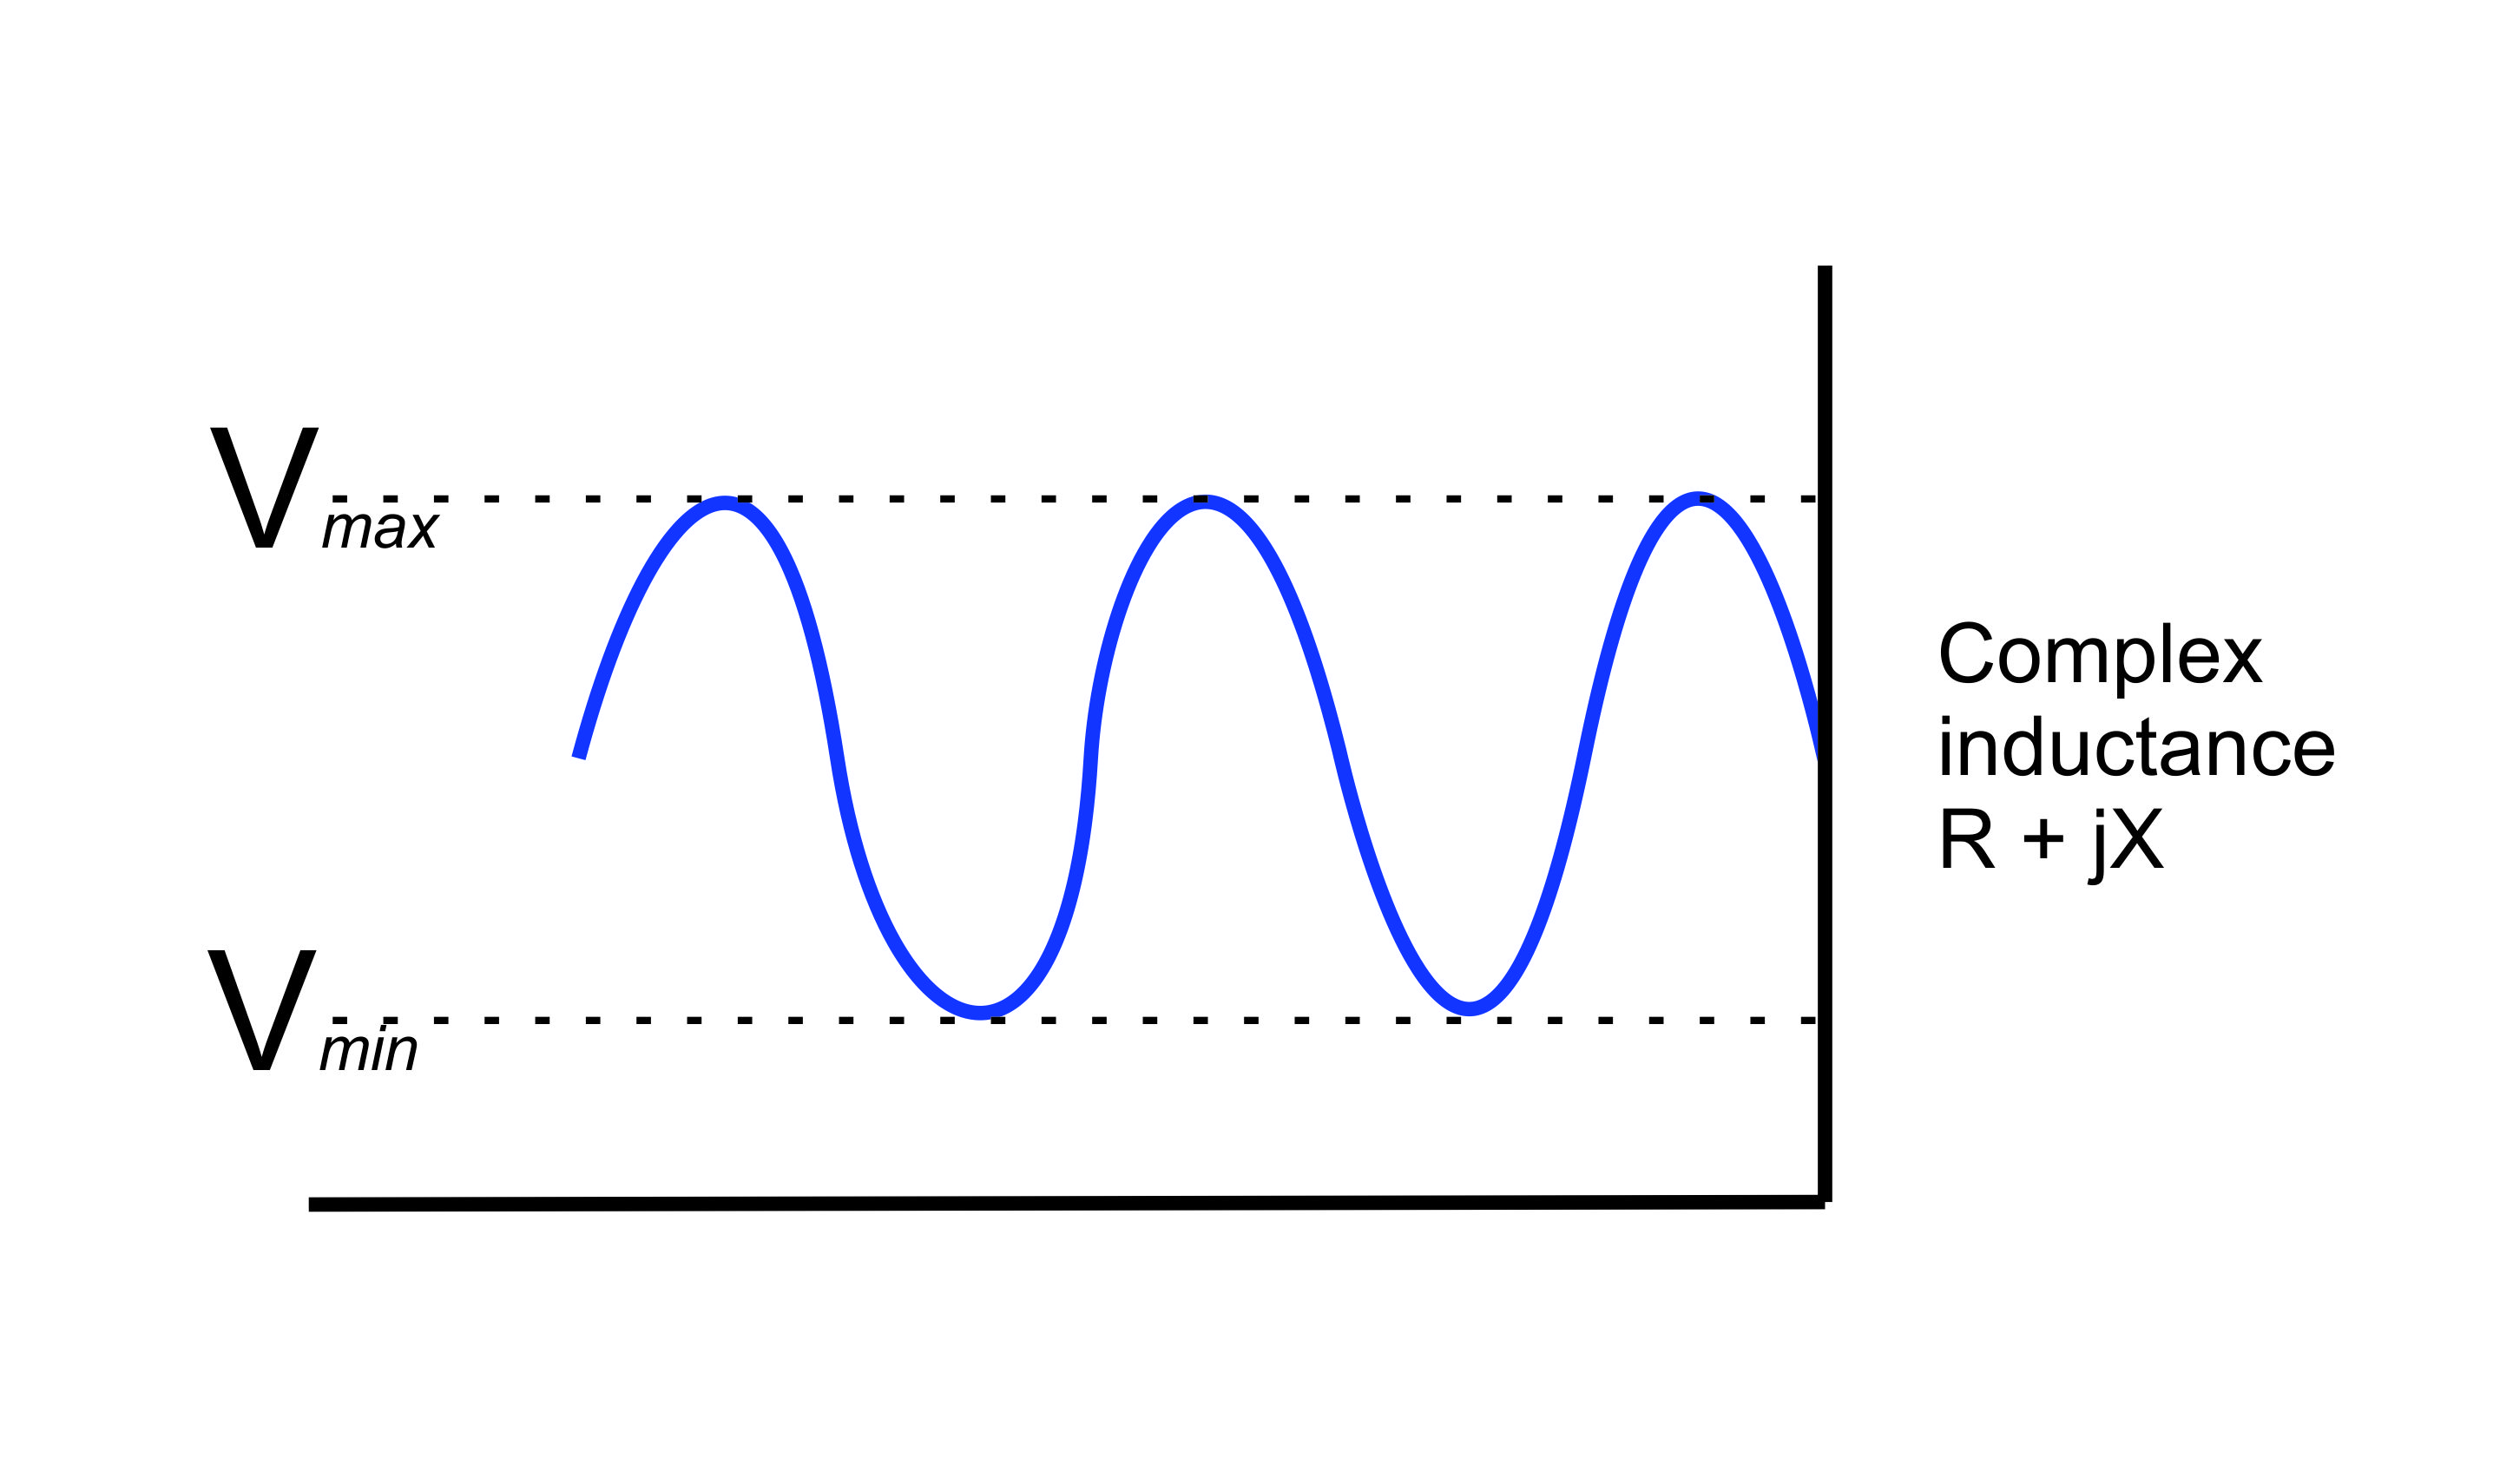
\includegraphics[width=0.8\linewidth]{\pathtopartone/graphics/Group93}
\caption{Standing wave pattern variation of a complex inductive load}
\label{fig:group93}
\end{figure}
\begin{figure}[h]
\centering
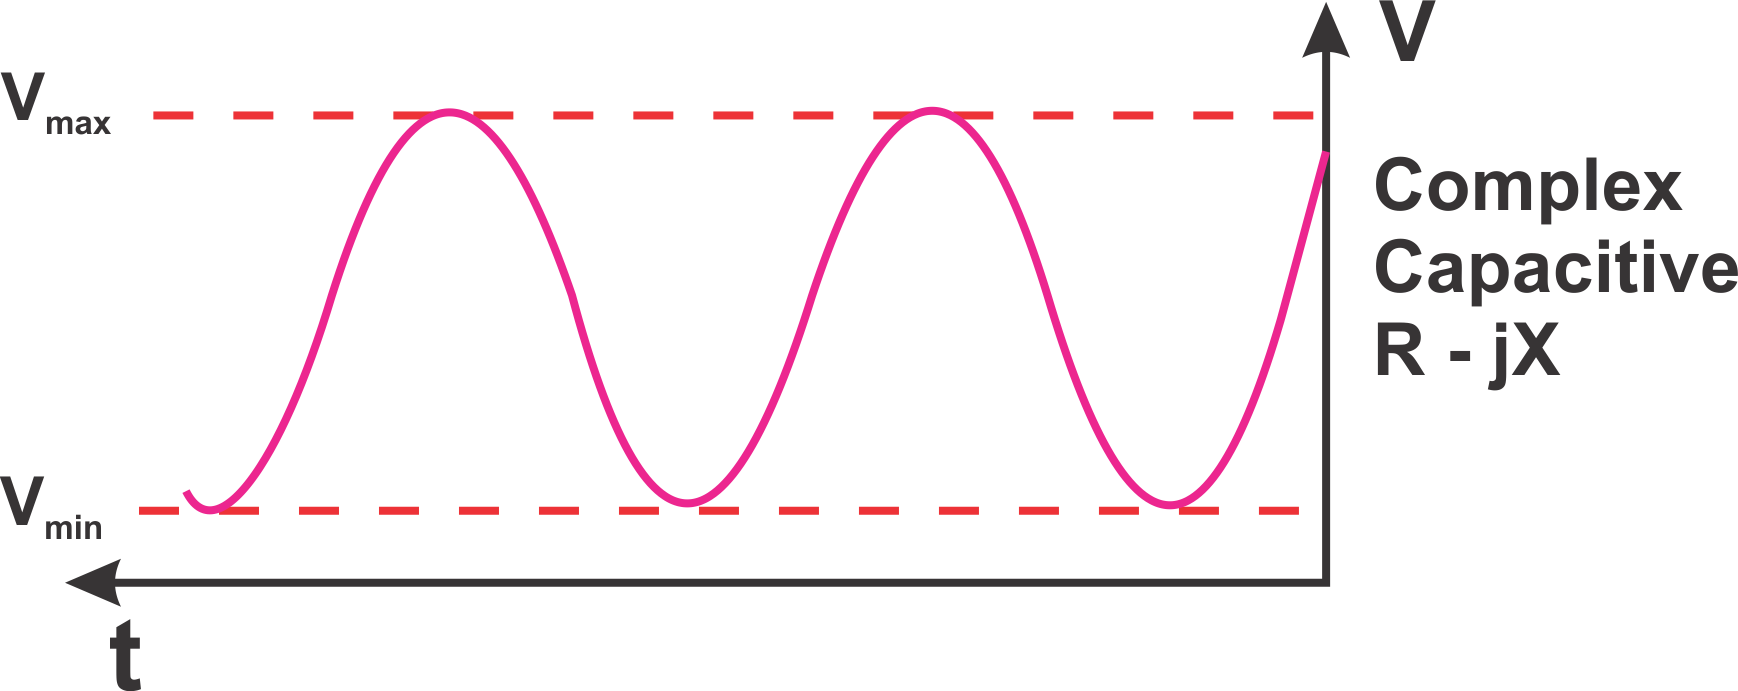
\includegraphics[width=0.8\linewidth]{\pathtopartone/graphics/Group94}
\caption{Standing wave pattern variation of a complex capacitive load}
\label{fig:group94}
\end{figure}

Similarly, for a complex capacitive load, $V_\min\neq0$ and we encounter $V_\min$ first before $V_\max$ as shown in figure~\ref{fig:group94}. 

\subsubsection{Purely Reactive Loads}
Let us observe the standing wave patterns with pure reactive components at the load end. As shown in figure~\ref{fig:group96}, the voltage minimum is zero or it touches the horizontal axis that is ${VSWR=\dfrac{V_\max}{V_\min}=\infty}$ as ${V_\min=0}$.
\begin{figure}[h]
\centering
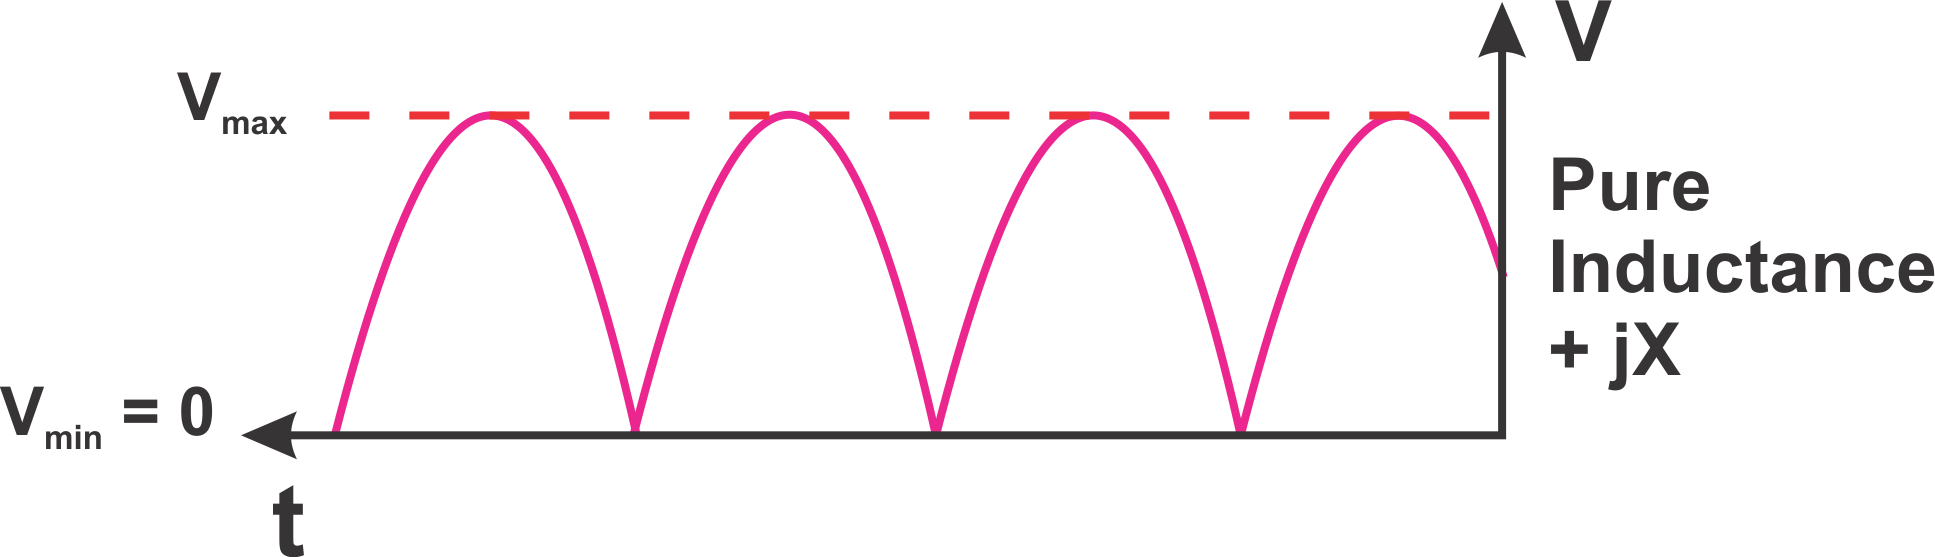
\includegraphics[width=0.8\linewidth]{\pathtopartone/graphics/Group96}
\caption{Standing wave pattern variation of a purely inductive load}
\label{fig:group96}
\end{figure}

As we move from the load end we meet ${V_\max}$ first indicating it is purely inductive and lies on the upper half of the Smith Chart.
\begin{figure}[h]
\centering
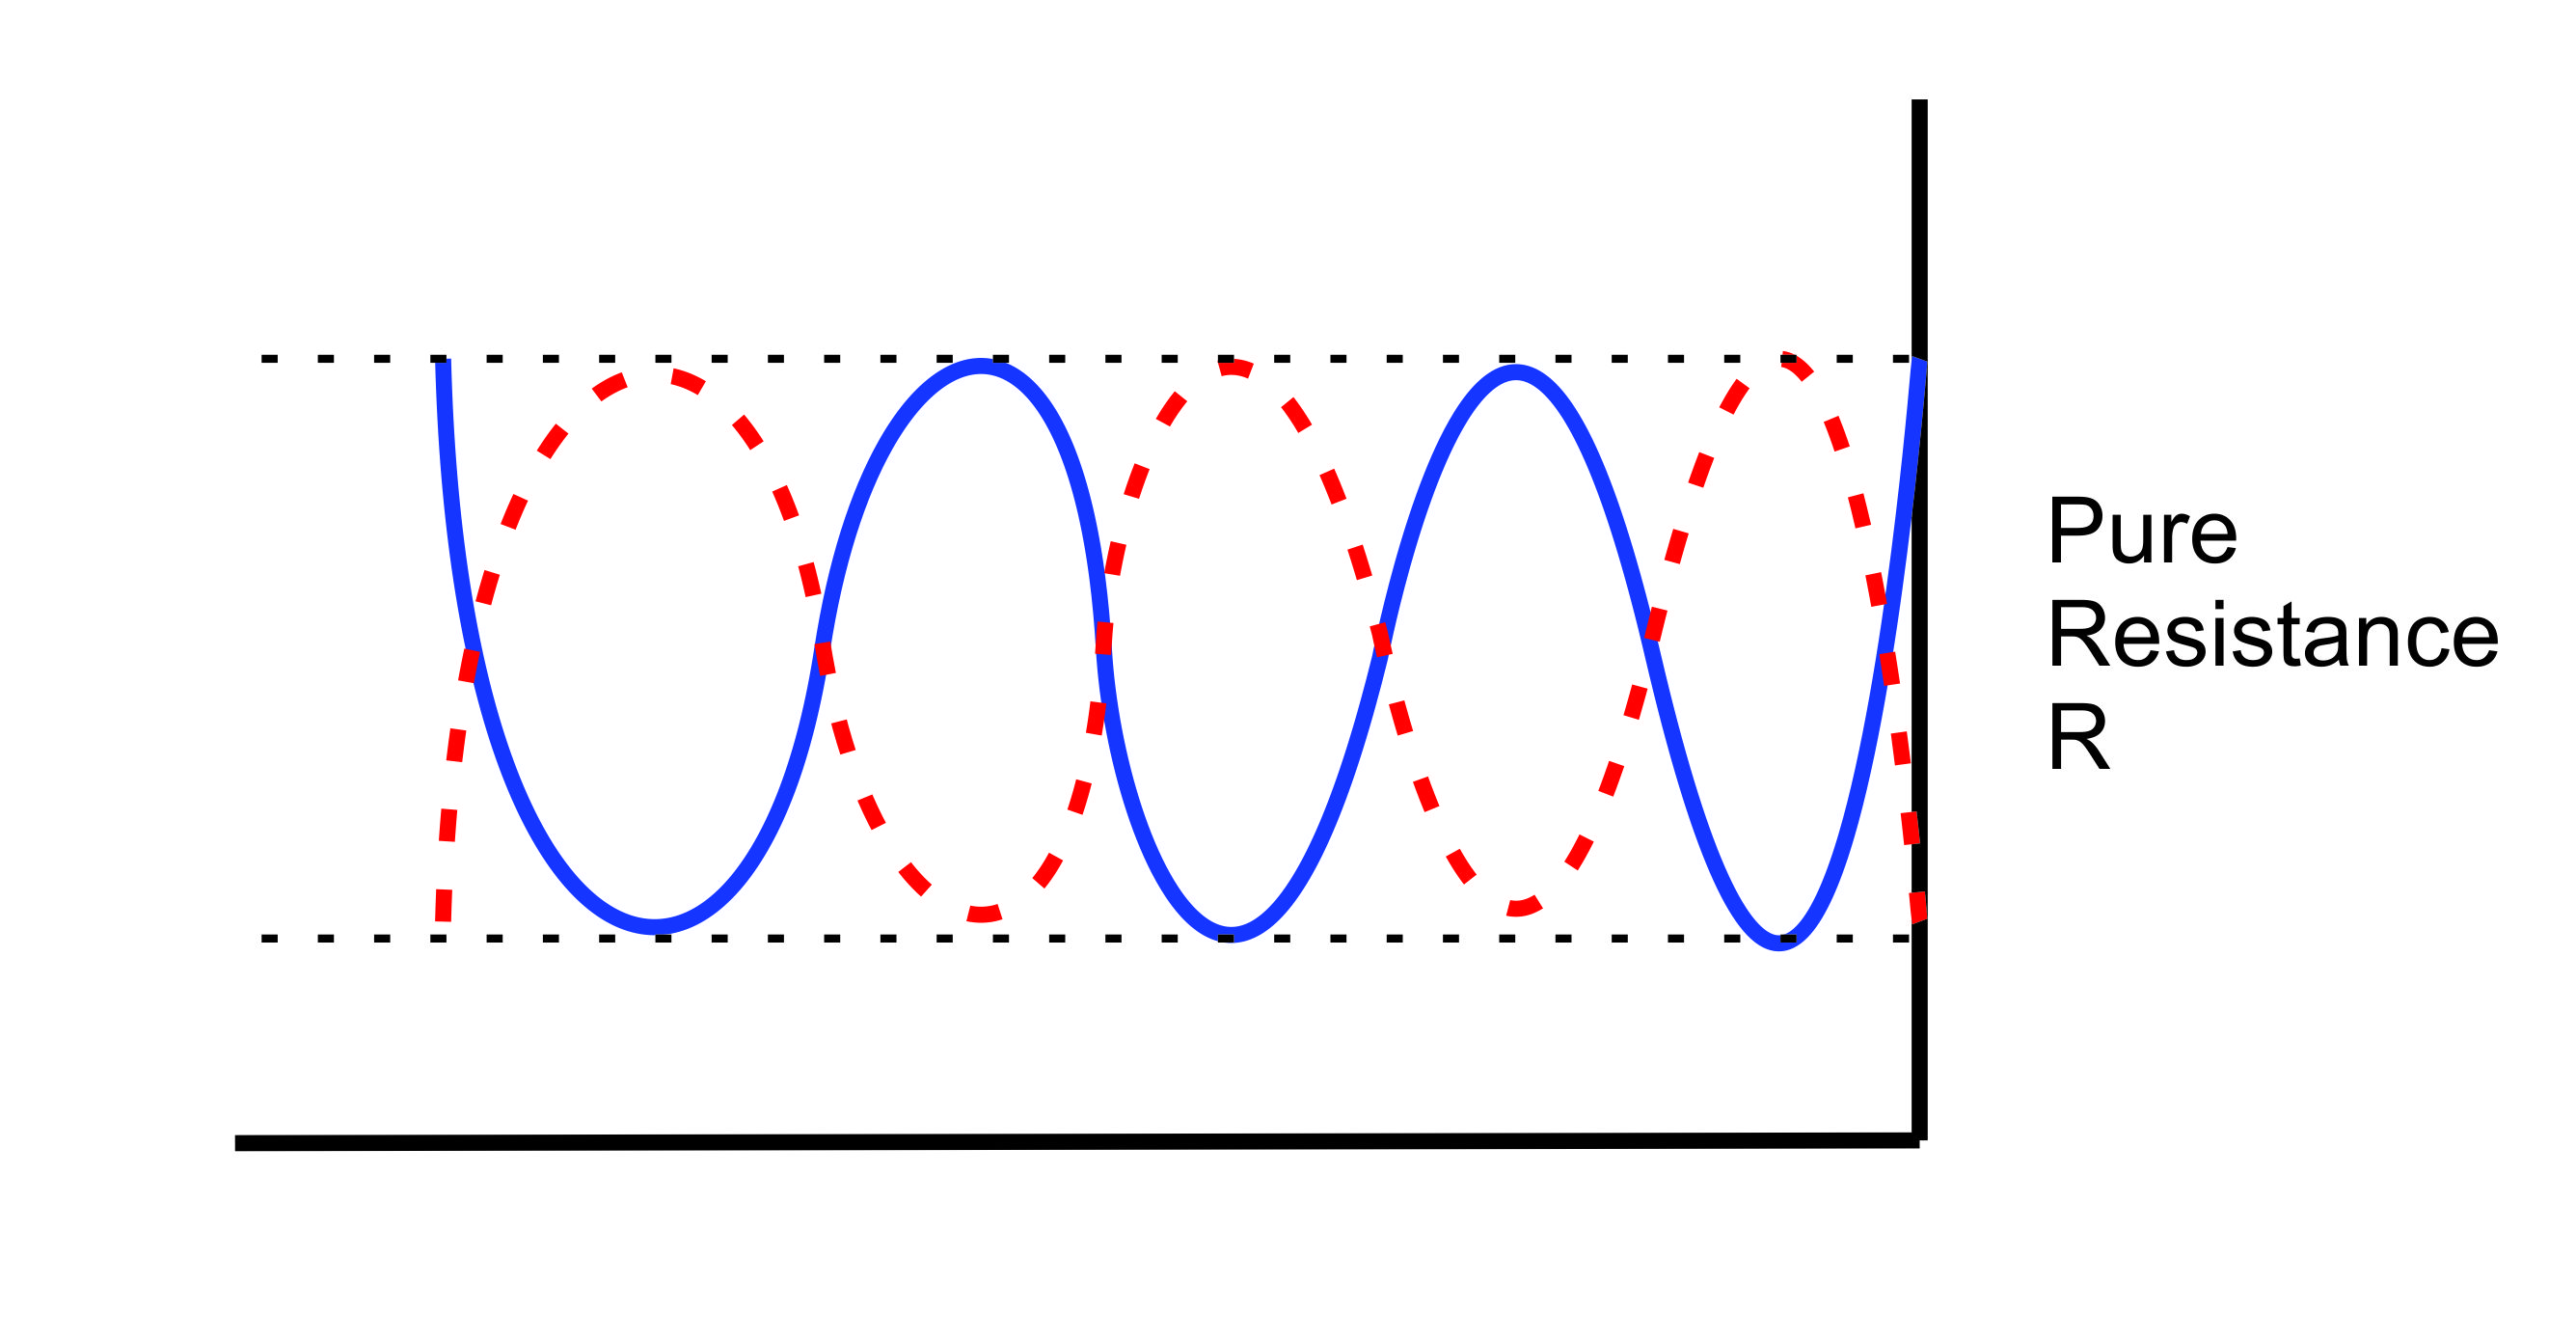
\includegraphics[width=0.8\linewidth]{\pathtopartone/graphics/Group97}
\caption{Standing wave pattern variation of a purely capacitive load}
\label{fig:group97}
\end{figure}

For purely capacitive loads, the voltage minimum is also zero, but we encounter a minimum first as we go from the load end towards the generator indicating a purely capacitive load. So it lies in the lower half of the Smith chart and $VSWR=\infty$.

\subsubsection{Resistive Loads}
Lastly, there is the case when the load is neither capacitive nor inductive. If so, then the load must lie on the real horizontal axis of the Smith Chart, so the location of the load itself will be at either the voltage minimum point or the voltage maximum point. If the load is purely resistive as in figure~\ref{fig:group95}. Recall that on the Smith Chart, the points of intersection of the VSWR circle on the real axis will be the locations of the voltage maximum and minimum. So there will either be maximum or minimum voltage at the load end as shown in figure~\ref{fig:group95}. The solid curve has ${V_\max}$ at load end meaning ${R>Z_0}$ while the dashed curve has ${V_\min}$ at load end which means ${R<Z_0}$. ${Z_0}$ is the characteristics impedance.
\begin{figure}[h]
\centering
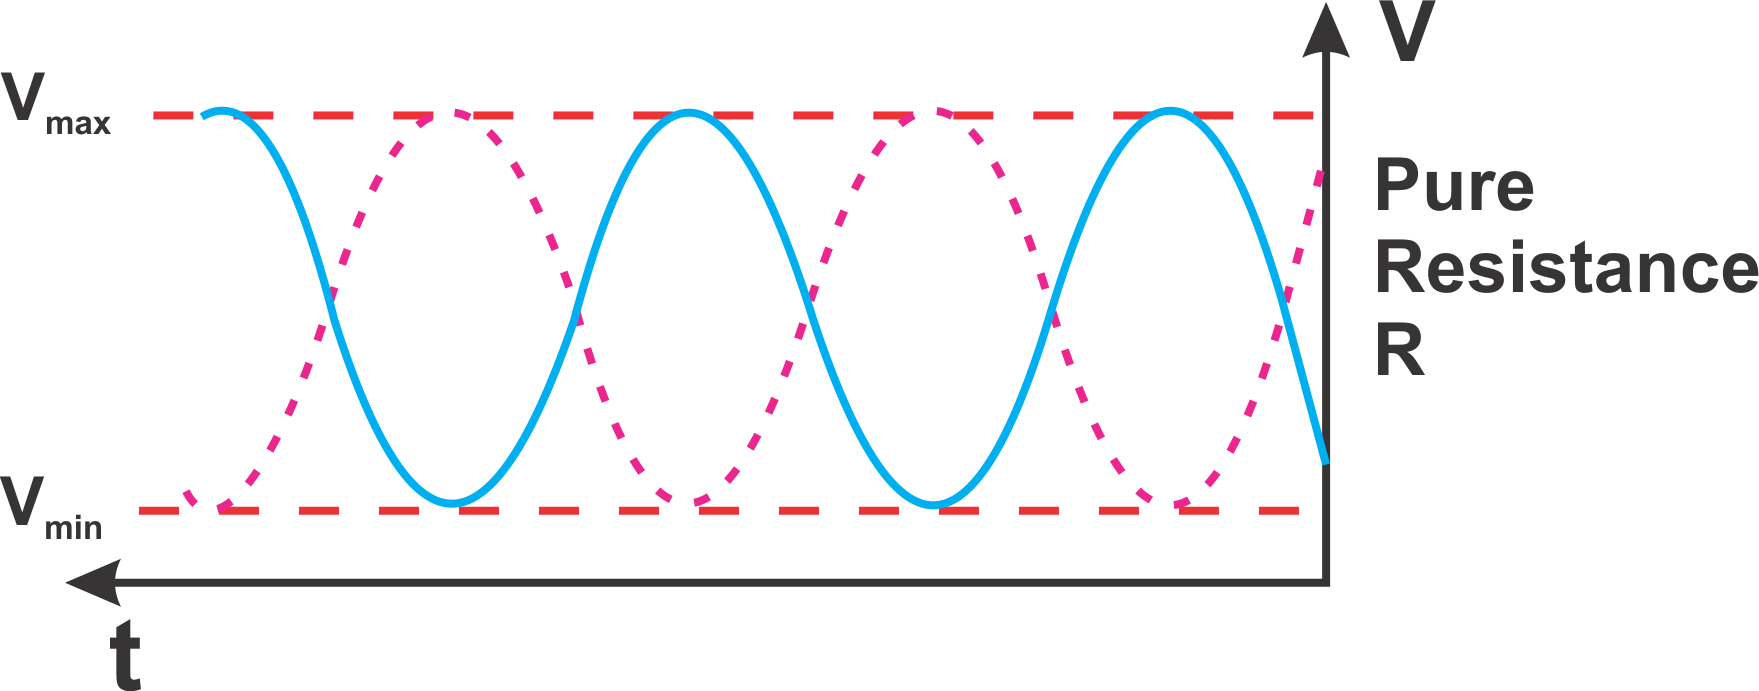
\includegraphics[width=0.8\linewidth]{\pathtopartone/graphics/Group95}
\caption{Standing wave pattern variation of a pure resistive}
\label{fig:group95}
\end{figure}

So looking at the standing wave pattern, one can quickly identify the types of loads because the information about the load is completely available from the standing wave pattern. Hence, ${V_\max}$ and ${V_\min}$ location and lowest value of ${V_\min}$ which is related to VSWR can help us identify loads very quickly.

So in this section, we have shown how to identify the load by looking at standing wave patterns. Next, we go to applications of transmission lines since we make use of sections of transmission lines in realizing various circuit elements in high-frequency circuits.

\section*{Exercises}
\begin{ExerciseList}
\Exercise[label={ex91}]
Explain the following:
\end{ExerciseList}